\appendix
\beginsupplement
\onecolumn

\begin{center}
    \Large\textbf{Supplementary Material\\Putting the Object Back into Video Object Segmentation}
\end{center}

The supplementary material is structured as follows:

\begin{enumerate}
    \item We first provide visual comparisons of Cutie with state-of-the-art methods in Section~\ref{sec:app:visual-comparisons}.
    \item We then show some highly challenging cases where both Cutie and state-of-the-art methods fail in Section~\ref{sec:app:failure-cases}.
    \item To elucidate the workings of the object transformer, we visualize the difference in attention patterns of pixel readout v.s.\ object readout, and feature progression within the object transformer in Section~\ref{sec:app:visualizations}.
    \item We list options for adjusting the speed-accuracy trade-off without re-training, comparisons with methods that use external training, additional quantitative results on YouTube-VOS 2018~\cite{xu2018youtubeVOS}/LVOS~\cite{hong2022lvos}, and the performance variations with respect to different random seeds in Section~\ref{sec:app:quantitative}.
    \item Lastly, we give more implementation details on the training process, decoder architecture, and pixel memory in Section~\ref{sec:app:implementation}.
\end{enumerate}

\section{Visual Comparisons}\label{sec:app:visual-comparisons}
We provide visual comparisons of Cutie with DeAOT-R50~\cite{yang2022decoupling} and XMem~\cite{cheng2022xmem} in the attached {\tt comparisons.mp4}.
For a fair comparison, we use Cutie-base and train all models with the MOSE dataset.
We visualize the comparisons using sequences from YouTubeVOS-2019 validation, DAVIS 2017 test-dev, and MOSE validation. 
Only the first-frame (not full-video) ground-truth annotations are available in these datasets. 
At the beginning of each sequence, we pause for two seconds to show the first-frame segmentation that initializes all the models.
Our model is more robust to distractors and generates more coherent masks.

\section{Failure Cases}\label{sec:app:failure-cases}
We visualize some failure cases of Cutie in {\tt failure\_cases.mp4}, following the format discussed in Section~\ref{sec:app:visual-comparisons}.
As discussed in the main paper, Cutie fails in some of the challenging cases where similar objects move in close proximity or occlude each other. 
This problem is not unique to Cutie, as current state-of-the-art methods also fail as shown in {\tt failure\_cases.mp4}.

In the first sequence ``elephants'', all models have difficulty tracking the elephants (e.g., light blue mask) behind the big (unannotated) foreground elephant.
In the second sequence ``birds'', all models fail when the bird with the pink mask moves and occludes other birds.

We think that this is due to the lack of useful features from the pixel memory and the object memory, as they fail to disambiguate objects that are similar in both appearance and position.
A potential future work direction for this is to encode three-dimensional spatial understanding (i.e., the bird that occludes is closer to the camera).

\section{Additional Visualizations}\label{sec:app:visualizations}
\subsection{Attention Patterns of Pixel Attention v.s.\ Object Query Attention}
Here, we visualize the attention maps of pixel memory reading and of the object transformer, showing the qualitative difference between the two.

To visualize attention in pixel memory reading, we use ``self-attention'', i.e., by setting .
We compute the pixel affinity , as in Equation (9) of the main paper.
We then sum over the foreground region along the rows, visualizing the affinity of every pixel to the foreground. Ideally, all the affinity should be in the foreground -- others are distractors that cause erroneous matching. The foreground region is defined by the last auxiliary mask  in the object transformer.

To visualize the attention in the object transformer, we inspect the attention weights  of the first (pixel-to-query) cross-attention in the last object transformer block.
Similar to how we visualize the pixel attention, we focus on the foreground queries (i.e., first  object queries) and sum over the corresponding rows in the affinity matrix.

Figure~\ref{fig:app:attn-weights} visualizes the differences between these two types of attention. The pixel attention is more spread out and is easily distracted by similar objects.
The object query attention focuses on the foreground without being distracted.
Our object transformer makes use of both types of attention by using pixel attention for initialization and object query attention for restructuring the feature in every transformer block.

\begin{figure}
    \centering
    \small


\begin{tabular}{c@{\hspace{4pt}}c@{\hspace{4pt}}c@{\hspace{4pt}}c}
    Input image &  Target object mask & Pixel attention map & Object query attention map \\
    \includegraphics[width=0.24\linewidth]{img/attention/image/00001.jpg} & 
    \includegraphics[width=0.24\linewidth]{img/attention/gt/00001.png} & 
    \includegraphics[width=0.24\linewidth]{img/attention/pix/00001_obj1.jpg} &
    \includegraphics[width=0.24\linewidth]{img/attention/ours/00001_obj1.jpg} \\ 
    \includegraphics[width=0.24\linewidth]{img/attention/image/00009.jpg} & 
    \includegraphics[width=0.24\linewidth]{img/attention/gt/00009.png} & 
    \includegraphics[width=0.24\linewidth]{img/attention/pix/00009_obj1.jpg} &
    \includegraphics[width=0.24\linewidth]{img/attention/ours/00009_obj1.jpg} \\
    \includegraphics[width=0.24\linewidth]{img/attention/image/00092.jpg} & 
    \includegraphics[width=0.24\linewidth]{img/attention/gt/00092.png} & 
    \includegraphics[width=0.24\linewidth]{img/attention/pix/00092_obj1.jpg} &
    \includegraphics[width=0.24\linewidth]{img/attention/ours/00092_obj1.jpg} \\
 \end{tabular}     \caption{Comparison of foreground attention patterns between pixel attention with object query attention. 
    In each of the three examples, the two leftmost columns show the input image and the ground-truth (annotated by us for reference).
    The two rightmost columns show the attention patterns for pixel attention and object query attention respectively.
    Ideally, the attention weights should focus on the foreground object. As shown, the pixel attention has a broader coverage but is easily distracted by similar objects.
    The object query attention's attention is more sparse (as we use a small number of object queries), and is more focused on the foreground. 
    Our object transformer makes use of both: it first initializes with pixel attention and restructures the features iteratively with object query attention.
    }
    \label{fig:app:attn-weights}
\end{figure}
\begin{figure}
    \centering
    \begin{tabular}{c@{\hspace{1pt}}c@{\hspace{1pt}}c@{\hspace{1pt}}c@{\hspace{1pt}}c}
Image & 
 &
 & 
 & 
Ground-truth \\
 \includegraphics[width=0.19\linewidth]{img/progression/image/00001.jpg} & 
 \includegraphics[width=0.19\linewidth]{img/progression/ours/00001_obj1_lvl1.png} & 
 \includegraphics[width=0.19\linewidth]{img/progression/ours/00001_obj1_lvl2.png} & 
 \includegraphics[width=0.19\linewidth]{img/progression/ours/00001_obj1_lvl3.png} & 
 \includegraphics[width=0.19\linewidth]{img/progression/gt/00001.png} \\
 \includegraphics[width=0.19\linewidth]{img/progression/image/00019.jpg} & 
 \includegraphics[width=0.19\linewidth]{img/progression/ours/00019_obj1_lvl1.png} & 
 \includegraphics[width=0.19\linewidth]{img/progression/ours/00019_obj1_lvl2.png} & 
 \includegraphics[width=0.19\linewidth]{img/progression/ours/00019_obj1_lvl3.png} & 
 \includegraphics[width=0.19\linewidth]{img/progression/gt/00019.png} \\
 \includegraphics[width=0.19\linewidth]{img/progression/image/00020.jpg} & 
 \includegraphics[width=0.19\linewidth]{img/progression/ours/00020_obj1_lvl1.png} & 
 \includegraphics[width=0.19\linewidth]{img/progression/ours/00020_obj1_lvl2.png} & 
 \includegraphics[width=0.19\linewidth]{img/progression/ours/00020_obj1_lvl3.png} & 
 \includegraphics[width=0.19\linewidth]{img/progression/gt/00020.png} \\
\end{tabular}     \caption{Visualization of auxiliary masks  in the -th object transformer block. At every layer, matching errors are suppressed (pink arrows) and the target object becomes more coherent (yellow arrows). The ground-truth is annotated by us for reference.}
    \label{fig:app:feature-progression}
\end{figure}

\subsection{Feature Progression in the Object Transformer}
Figure~\ref{fig:app:feature-progression} visualizes more feature progression within the object transformer (in addition to Figure~4 in the main paper).
The object transformer helps to suppress noises from low-level matching and produces more coherent object-level features.

\clearpage
\section{Additional Quantitative Results}\label{sec:app:quantitative}

\subsection{Speed-Accuracy Trade-off}
We note that the performance of Cutie can be further improved by changing hyperparameters like memory interval and the size of the memory bank during inference, at the cost of a slower running time.
Here, we present ``Cutie+'', which adjusts the following hyperparameters without re-training:
\begin{enumerate}
    \item Maximum memory frames 
    \item Memory interval 
    \item Maximum shorter side resolution during inference  pixels
\end{enumerate}
These settings apply to DAVIS~\cite{perazzi2016benchmark} and MOSE~\cite{ding2023mose}. 
For YouTubeVOS, we keep the memory interval  and set the maximum shorter side resolution during inference to  for two reasons: 1) YouTubeVOS is annotated every 5 frames, and aligning the memory interval with annotation avoids adding unannotated objects into the memory as background, and 2) YouTubeVOS has lower video quality and using higher resolution makes artifacts more apparent.
The results of Cutie+ are tabulated in the bottom portion of Table~\ref{tab:app:external-training}. 

\subsection{Comparisons with Methods that Use External Training}

\begin{table}
    \small
\centering
\begin{NiceTabular}
{l@{\hspace{2pt}}l@{\hspace{6pt}}C{2.2em}@{}C{2.2em}@{}C{2.2em}@{\hspace{5pt}}C{2.2em}@{}C{2.2em}@{}C{2.2em}@{\hspace{5pt}}C{2.2em}@{}C{2.2em}@{}C{2.2em}@{\hspace{5pt}}C{2.2em}@{}C{2.2em}@{}C{2.2em}@{}C{2.2em}@{}C{2.2em}@{}R{2em}}[colortbl-like]
\toprule
&& \multicolumn{3}{c}{\small MOSE} & \multicolumn{3}{c}{\small DAVIS-17 val} & \multicolumn{3}{c}{\small DAVIS-17 test} & \multicolumn{6}{c}{\small YouTubeVOS-2019 val} \\
\cmidrule(lr{\dimexpr 4\tabcolsep+8pt}){3-6} \cmidrule(lr{\dimexpr 4\tabcolsep+8pt}){6-9} \cmidrule(lr{\dimexpr 4\tabcolsep+8pt}){9-12} \cmidrule(lr){12-17}
Method && \mjf & \mj & \mf & \mjf & \mj & \mf & \mjf & \mj & \mf & \mg & \mjs & \mfs & \mju & \mfu & FPS \\
\toprule
SimVOS-B~\cite{wu2023scalable} &  & - & - & - & 81.3 & 78.8 & 83.8 & - & - & - & - & - & - & - & - & 3.3 \\
SimVOS-B~\cite{wu2023scalable} & w/ MAE~\cite{he2021masked} & - & - & - & 88.0 & 85.0 & 91.0 & 80.4 & 76.1 & 84.6 & 84.2 & 83.1 & - & 79.1 & - & 3.3 \\
JointFormer~\cite{zhang2023joint} &  & - & - & - & - & - & - & 65.6 & 61.7 & 69.4 & 73.3 & 75.2 & 78.5 & 65.8 & 73.6 & 3.0 \\
JointFormer~\cite{zhang2023joint} & w/ MAE~\cite{he2021masked}  & - & - & - & 89.7 & 86.7 & 92.7 & 87.6 & 84.2 & 91.1 & 87.0 & 86.1 & 90.6 & 82.0 & 89.5 & 3.0 \\
JointFormer~\cite{zhang2023joint} & w/ MAE~\cite{he2021masked} + BL30K~\cite{cheng2021mivos} & - & - & - & 90.1 & 87.0 & \textbf{93.2} & \textbf{88.1} & \textbf{84.7} & \textbf{91.6} & \textbf{87.4} & \textbf{86.5} & \textbf{90.9} & 82.0 & \textbf{90.3} & 3.0 \\
ISVOS~\cite{wang2022look} & & - & - & - & 80.0 & 76.9 & 83.1 & - & - & - & - & - & - & - & - & 5.8  \\
ISVOS~\cite{wang2022look} & w/ COCO~\cite{lin2014microsoft} & - & - & - & 87.1 & 83.7 & 90.5 & 82.8 & 79.3 & 86.2 & 86.1 & 85.2 & 89.7 & 80.7 & 88.9 & 5.8  \\
ISVOS~\cite{wang2022look} & w/ COCO~\cite{lin2014microsoft} + BL30K~\cite{cheng2021mivos} & - & - & - & 88.2 & 84.5 & 91.9 & 84.0 & 80.1 & 87.8 & 86.3 & 85.2 & 89.7 & 81.0 & 89.1 & 5.8  \\
\rowcolor{defaultColor}
Cutie-small & & 62.2 & 58.2 & 66.2 & 87.2 & 84.3 & 90.1 & 84.1 & 80.5 & 87.6 & 86.2 & 85.3 & 89.6 & 80.9 & 89.0 & \textbf{45.5} \\
\rowcolor{defaultColor}
Cutie-base & & 64.0 & 60.0 & 67.9 & 88.8 & 85.4 & 92.3 & 84.2 & 80.6 & 87.7 & 86.1 & 85.5 & 90.0 & 80.6 & 88.3 & 36.4 \\
\midrule
\rowcolor{defaultColor}
Cutie-small & w/ MOSE~\cite{ding2023mose} & 67.4 & 63.1 & 71.7 & 86.5 & 83.5 & 89.5 & 83.8 & 80.2 & 87.5 & 86.3 & 85.2 & 89.7 & 81.1 & 89.2 & \textbf{45.5} \\
\rowcolor{defaultColor}
Cutie-base & w/ MOSE~\cite{ding2023mose} & 68.3 & 64.2 & 72.3 & 88.8 & 85.6 & 91.9 & 85.3 & 81.4 & 89.3 & 86.5 & 85.4 & 90.0 & 81.3 & 89.3 & 36.4 \\
\rowcolor{defaultColor}
Cutie-small & w/ MEGA & 68.6 & 64.3 & 72.9 & 87.0 & 84.0 & 89.9 & 85.3 & 81.4 & 89.2 & 86.8 & 85.2 & 89.6 & 82.1 & \textbf{90.4} & \textbf{45.5} \\
\rowcolor{defaultColor}
Cutie-base & w/ MEGA & 69.9 & 65.8 & 74.1 & 87.9 & 84.6 & 91.1 & 86.1 & 82.4 & 89.9 & 87.0 & 86.0 & 90.5 & 82.0 & 89.6 & 36.4 \\
\rowcolor{defaultColor}
Cutie-small+ & & 64.3 & 60.4 & 68.2 & 88.7 & 86.0 & 91.3 & 85.7 & 82.5 & 88.9 & 86.7 & 85.7 & 89.8 & 81.7 & 89.6 & 20.6 \\
\rowcolor{defaultColor}
Cutie-base+ & & 66.2 & 62.3 & 70.1 & \textbf{90.5} & \textbf{87.5} & \textbf{93.4} & 85.9 & 82.6 & 89.2 & 86.9 & 86.2 & 90.7 & 81.6 & 89.2 & 17.9 \\
\rowcolor{defaultColor}
Cutie-small+ & w/ MOSE~\cite{ding2023mose} & 69.0 & 64.9 & 73.1 & 89.3 & 86.4 & 92.1 & 86.7 & 83.4 & 90.1 & 86.5 & 85.4 & 89.7 & 81.6 & 89.2 & 20.6 \\
\rowcolor{defaultColor}
Cutie-base+ & w/ MOSE~\cite{ding2023mose} & 70.5 & 66.5 & 74.6 & 90.0 & 87.1 & 93.0 & 86.3 & 82.9 & 89.7 & 86.8 & 85.7 & 90.0 & 81.8 & 89.6 & 17.9 \\
\rowcolor{defaultColor}
Cutie-small+ & w/ MEGA & 70.3 & 66.0 & 74.5 & 89.3 & 86.2 & 92.5 & 87.1 & 83.8 & 90.4 & 86.8 & 85.4 & 89.5 & 82.3 & 90.0 & 20.6 \\
\rowcolor{defaultColor}
Cutie-base+ & w/ MEGA & \textbf{71.7} & \textbf{67.6} & \textbf{75.8} & 88.1 & 85.5 & 90.8 & \textbf{88.1} & \textbf{84.7} & \textbf{91.4} & \textbf{87.5} & \textbf{86.3} & 90.6 & \textbf{82.7} & \textbf{90.5} & 17.9 \\
\midrule
\bottomrule
\end{NiceTabular}     \caption{Quantitative comparison on common video object segmentation benchmarks, including methods that use external training data.
    Recent vision-transformer-based methods~\cite{wang2022look,wu2023scalable,zhang2023joint} depend largely on pretraining, either with MAE~\cite{he2021masked} or pretraining a separate Mask2Former~\cite{cheng2022masked} network on COCO instance segmentation~\cite{lin2014microsoft}.
    Note they do not release code at the time of writing, and thus they cannot be reproduced on datasets that they do not report results on. 
    Cutie performs competitively to those recent (slow) transformer-based methods, especially with added training data.
    MEGA is the aggregated dataset consisting of DAVIS~\cite{perazzi2016benchmark}, YouTubeVOS~\cite{xu2018youtubeVOS}, MOSE~\cite{ding2023mose}, OVIS~\cite{qi2022occluded}, and BURST~\cite{athar2023burst}.
    estimated FPS.}
    \label{tab:app:external-training}
\end{table}

Here, we present comparisons with methods that use external training: SimVOS~\cite{shi2015hierarchicalECSSD}, JointFormer~\cite{zhang2023joint}, and ISVOS~\cite{wang2022look} in Table~\ref{tab:app:external-training}. 
Note, we could not obtain the code for these methods at the time of writing. 
ISVOS~\cite{wang2022look} does not report running time -- we estimate to the best of our ability with the following information: 
1) For the VOS branch, it uses XMem~\cite{cheng2022xmem} as the baseline with a first-in-first-out 16-frame memory bank, 
2) for the instance branch, it uses Mask2Former~\cite{cheng2022masked} with an unspecified backbone. Beneficially for ISVOS, we assume the lightest backbone (ResNet-50), and 
3) the VOS branch and the instance branch share a feature extraction backbone.
Our computation is as follows:
\begin{enumerate}
    \item Time per frame for XMem with a 16-frame first-in-first-out memory bank (from our testing): 75.2 ms
    \item Time per frame for Mask2Former with ResNet-50 backbone (from Mask2Former paper): 103.1 ms
    \item Time per frame of the doubled-counted feature extraction backbone (from our testing): 6.5 ms
\end{enumerate}
Thus, we estimate that ISVOS would take (75.2+103.1-6.5) = 171.8 ms per frame, which translates to 5.8 frames per second.

In an endeavor to reach a better performance with Cutie by adding more training data, we devise a ``MEGA'' training scheme that includes training on BURST~\cite{athar2023burst} and OVIS~\cite{qi2022occluded} in addition to DAVIS~\cite{perazzi2016benchmark}, YouTubeVOS~\cite{xu2018youtubeVOS}, and MOSE~\cite{ding2023mose}. 
We train for an additional 50K iterations in the MEGA setting.
The results are tabulated in the bottom portion of Table~\ref{tab:app:external-training}. 

\subsection{Results on YouTubeVOS-2018 and LVOS}\label{sec:app:lvos}

\begin{table}
    \centering
\begin{NiceTabular}
{l@{\hspace{2pt}}l@{\hspace{6pt}}C{2.2em}@{}C{2.2em}@{}C{2.2em}@{}C{2.2em}@{}C{2.2em}@{\hspace{5pt}}C{2.2em}@{}C{2.2em}@{}C{2.2em}@{\hspace{5pt}}C{2.2em}@{}C{2.2em}@{}C{2.2em}@{\hspace{5pt}}R{2em}}[colortbl-like]
\toprule
&& \multicolumn{5}{c}{\small YouTubeVOS-2018 val} & \multicolumn{3}{c}{\small LVOS val} & \multicolumn{3}{c}{\small LVOS test} & \\
\cmidrule(lr{\dimexpr 4\tabcolsep+8pt}){3-8} \cmidrule(lr{\dimexpr 4\tabcolsep+8pt}){8-11} \cmidrule(lr{\dimexpr 4\tabcolsep+8pt}){11-14} 
Method && \mg & \mjs & \mfs & \mju & \mfu & \mjf & \mj & \mf & \mjf & \mj & \mf & FPS \\
\midrule
DEVA~\cite{cheng2023tracking} &  & 85.9 & 85.5 & 90.1 & 79.7 & 88.2 & 58.3 & 52.8 & 63.8 & 54.0 & 49.0 & 59.0 & 25.3\\
DEVA~\cite{cheng2023tracking} & w/ MOSE~\cite{ding2023mose} & 85.8 & 85.4 & 90.1 & 79.7 & 88.2 & 55.9 & 51.1 & 60.7 & 56.5 & 52.2 & 60.8 & 25.3 \\
DDMemory~\cite{hong2022lvos} & & 84.1 & 83.5 & 88.4 & 78.1 & 86.5 & \textbf{60.7} & 55.0 & \textbf{66.3} & 55.0 & 49.9 & 60.2 & 18.7 \\
\rowcolor{defaultColor}
Cutie-small & & \textbf{86.3} & 85.5 & 90.1 & \textbf{80.6} & \textbf{89.0} & 58.8 & 54.6 & 62.9 & \textbf{57.2} & \textbf{53.7} & \textbf{60.7} & \textbf{45.5}\\
\rowcolor{defaultColor}
Cutie-base & & 86.1 & \textbf{85.8} & \textbf{90.5} & 80.0 & 88.0 & 60.1 & \textbf{55.9} & 64.2 & 56.2 & 51.8 & 60.5 & 36.4 \\
\midrule
\rowcolor{defaultColor}
Cutie-small & w/ MOSE~\cite{ding2023mose} & 86.8 & 85.7 & 90.4 & 81.6 & 89.7 & 60.7 & 55.6 & 65.8 & 56.9 & 53.5 & 60.2  & \textbf{45.5}\\
\rowcolor{defaultColor}
Cutie-base & w/ MOSE~\cite{ding2023mose} & 86.6 & 85.7 & 90.6 & 80.8 & 89.1 & 63.5 & 59.1 & 67.9 & 63.6 & 59.1 & 68.0 & 36.4  \\
\rowcolor{defaultColor}
Cutie-small & w/ MEGA & \textbf{86.9} & 85.5 & 90.1 & \textbf{81.7} & \textbf{90.2} & 62.9 & 58.3 & 67.4 & 66.4 & 61.9 & 70.9  & \textbf{45.5}\\
\rowcolor{defaultColor}
Cutie-base & w/ MEGA & \textbf{87.0} & \textbf{86.4} & \textbf{91.1} & 81.4 & 89.2 & \textbf{66.0} & \textbf{61.3} & \textbf{70.6} & \textbf{66.7} & \textbf{62.4} & \textbf{71.0} & 36.4  \\
\midrule
\bottomrule
\end{NiceTabular}     \caption{Quantitative comparison on YouTubeVOS-2018~\cite{xu2018youtubeVOS} and LVOS~\cite{hong2022lvos}. 
    DDMemory~\cite{hong2022lvos} is the baseline method presented in LVOS~\cite{hong2022lvos} with no available official code at the time of writing.
    Note, we think LVOS is significantly different than other datasets because it contains a lot more tiny objects. See Section~\ref{sec:app:lvos} for details.
    MEGA is the aggregated dataset consisting of DAVIS~\cite{perazzi2016benchmark}, YouTubeVOS~\cite{xu2018youtubeVOS}, MOSE~\cite{ding2023mose}, OVIS~\cite{qi2022occluded}, and BURST~\cite{athar2023burst}.
    }
    \label{tab:app:lvos-results}
\end{table}

Here, we provide additional results on the YouTubeVOS-2018 validation set and LVOS~\cite{hong2022lvos} validation/test sets in Table~\ref{tab:app:lvos-results}.
FPS is measured on YoutubeVOS-2018/2019 following the main paper.
YouTubeVOS-2018 is the old version of YouTubeVOS-2019 -- we present our main results using YouTubeVOS-2019 and provide results on YouTubeVOS-2018 for reference.

LVOS~\cite{hong2022lvos} is a recently proposed long-term video object segmentation benchmark, with 50 videos in its validation set and test set respectively.
Note, we have also presented results in another long-term video object segmentation benchmark, BURST~\cite{athar2023burst} in the main paper, which contains 988 videos in the validation set and 1419 videos in the test set.
We test Cutie on LVOS \emph{after} completing the design of Cutie, and perform no tuning.
We note that our method (Cutie-base) performs better than DDMemory, the baseline presented in LVOS~\cite{hong2022lvos}, on the test set and has a comparable performance on the validation set, while running about twice as fast.
Upon manual inspection of the results, we observe that one of the unique challenges in LVOS is the prevalence of tiny objects, which our algorithm has not been specifically designed to handle.
We quantify this observation by analyzing the first frame annotations of all the videos in the validation sets of DAVIS~\cite{perazzi2016benchmark}, YouTubeVOS~\cite{xu2018youtubeVOS}, MOSE~\cite{ding2023mose}, BURST~\cite{athar2023burst}, and LVOS~\cite{hong2022lvos}, as shown in Figure~\ref{fig:app:lvos-object-sizes}.
Tiny objects are significantly more prevalent on LVOS~\cite{hong2022lvos} than on other datasets.
We think this makes LVOS uniquely challenging for methods that are not specifically designed to detect small objects.

\begin{figure}
    \centering
    \includegraphics[width=\linewidth]{plots/object_sizes.pdf}
    \caption{Cumulative frequency graph of annotated pixel areas (as percentages of the total image area) for different datasets.
    Tiny objects are significantly more prevalent on LVOS~\cite{hong2022lvos} than on other datasets.}
    \label{fig:app:lvos-object-sizes}
\end{figure}

\subsection{Performance Variations}
To assess performance variations with respect to different random seeds, we train Cutie-small with five different random seeds (including both pretraining and main training with the MOSE dataset) and report medianstandard deviation on the MOSE~\cite{ding2023mose} validation set and the YouTubeVOS 2019~\cite{xu2018youtubeVOS} validation set in Table~\ref{tab:app:random-variations}.
Note, the improvement brought by our model (i.e., 8.7~\mjf~on MOSE and 0.9~\mg~on YouTubeVOS over XMem~\cite{cheng2022xmem}) corresponds to  and  respectively.

\begin{table}
    \centering
    \centering
\begin{tabular}
{C{2.2em}@{\hspace{6pt}}C{2.2em}@{\hspace{6pt}}C{2.2em}@{\hspace{6pt}}C{2.2em}@{\hspace{6pt}}C{2.2em}@{\hspace{6pt}}C{2.2em}@{\hspace{6pt}}C{2.2em}@{\hspace{6pt}}C{2.2em}}
\toprule
\multicolumn{3}{c}{\hspace{-10pt}MOSE val\hspace{10pt}} & \multicolumn{5}{c}{YouTubeVOS-2019 val} \\
\cmidrule(lr){1-3} \cmidrule(lr){4-8}
\mjf & \mj & \mf & \mg & \mjs & \mfs & \mju & \mfu \\
\midrule
67.30.36 & 63.10.36 & 71.60.35 & 86.20.11 & 85.20.20 & 89.70.27 & 81.20.19 & 89.20.13 \\
\midrule
\bottomrule
\end{tabular}     \caption{Performance variations (medianstandard deviation) across five different random seeds.}
    \label{tab:app:random-variations}
\end{table}


\section{Implementation Details}\label{sec:app:implementation}
Here, we include more implementation details for completeness. 
Our training and testing code will be released for reproducibility.

\subsection{Extension to Multiple Objects}
We extend Cutie to the multi-object setting following~\cite{oh2019videoSTM,cheng2021stcn,cheng2022xmem,cheng2023tracking}. 
Objects are processed independently (in parallel as a batch) except for 
1) the interaction at the first convolutional layer of the mask encoder, which extracts features corresponding to a target object with a 5-channel input concatenated from the image (3-channel), the mask of the target object (1-channel), and the sum of masks of all non-target objects (1-channel); 
2) the interaction at the soft-aggregation layers~\cite{oh2019videoSTM} used to generate segmentation logits -- where the object probability distributions at every pixel are normalized to sum up to one. 
Note these are standard operations from prior works~\cite{oh2019videoSTM,cheng2021stcn,cheng2022xmem,cheng2023tracking}.
Parts of the computation (i.e., feature extraction from the query image and affinity computation) are shared between objects while the rest are not. 
We experimented with object interaction within the object transformer in the early stage of this project but did not obtain positive results. 

Figure~\ref{fig:app:plot-fps_vs_num_objects} plots the FPS against the number of objects. 
Our method slows down with more objects but remains real-time when handling a common number of objects in a scene (29.9 FPS with 5 objects). 
For instance, the BURST~\cite{athar2023burst} dataset averages 5.57 object tracks per video and DAVIS-2017~\cite{perazzi2016benchmark} averages just 2.03.

Additionally, we plot the memory usage with respect to the number of processed frames during inference in Figure~\ref{fig:app:plot-mem_vs_length}.

\begin{figure}
    \centering
    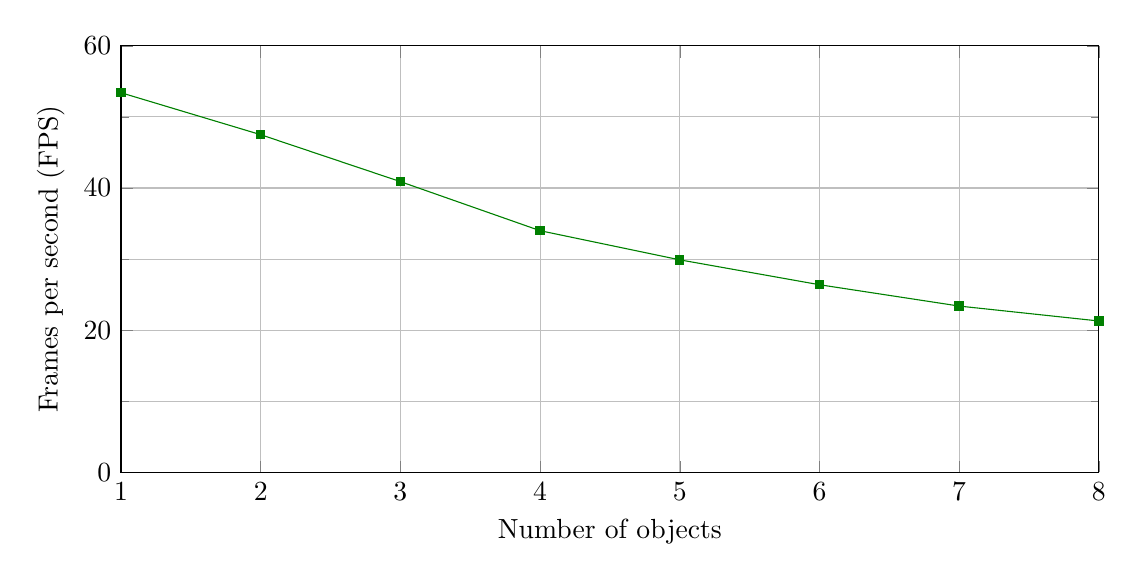
\begin{tikzpicture}
	\begin{axis}[
		xlabel={Number of objects},
		ylabel={Frames per second (FPS)},
		xmin=1, xmax=8,
		ymin=0, ymax=60,
        yminorticks=true,
        minor y tick num=1,
		grid=both,
		height=7cm, width=14cm,
        xtick={1, 2, 3, 4, 5, 6, 7, 8},
]
				\addplot[mark=*,mark=square*,color=Green,mark size=1.5pt]
		coordinates {
(1),(53.4)
(2),(47.5)
(3),(40.9)
(4),(34.0)
(5),(29.9)
(6),(26.4)
(7),(23.4)
(8),(21.3)
		};
  
	\end{axis}
\end{tikzpicture}     \caption{Cutie-small's processing speed with respect to the number of objects in the video. Common benchmarks (DAVIS~\cite{perazzi2016benchmark}, YouTubeVOS~\cite{xu2018youtubeVOS}, and MOSE~\cite{ding2023mose}) average 2-3 objects per video with longer-term benchmarks like BURST~\cite{athar2023burst} averaging 5.57 objects per video -- our model remains real-time (25+ FPS) in these scenarios.
    For evaluation, we use standard  test videos with 100 frames each.
    }
\label{fig:app:plot-fps_vs_num_objects}
\end{figure}

\subsection{Streaming Average Algorithm for the Object Memory}
To recap, we store a compact set of  vectors which make up a high-level summary of the target object in the object memory .
At a high level, we compute  by mask-pooling over all encoded object features with  different masks. Concretely, given object features  and  pooling masks , where  is the number of memory frames, the -th object memory  is computed by


During inference, we use a classic streaming average algorithm such that this operation takes constant time and memory with respect to the memory length. 
Concretely, for the -th object memory at time step , we keep track of a cumulative memory  and a cumulative weight . 
We update the accumulators and find  via

where  and  can be discarded after every time step.

\begin{figure}
    \centering
    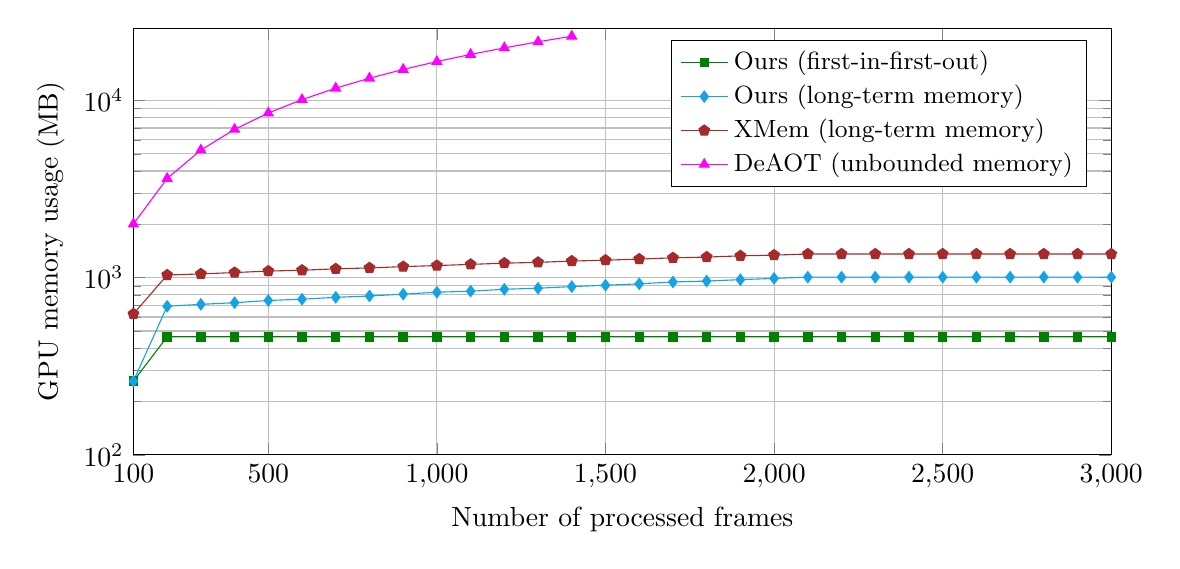
\begin{tikzpicture}
	\begin{axis}[
		xlabel={Number of processed frames},
		ylabel={GPU memory usage (MB)},
		xmin=100, xmax=3000,
        ymode=log,
		ymin=100, ymax=25600,
        yminorticks=true,
xtick={100, 500, 1000, 1500, 2000, 2500, 3000},
		grid=both,
		height=7cm, width=14cm,
		legend style={font=\small,at={(0.55,0.8)},anchor=west},
		legend cell align={left},
		]
				\addplot[mark=*,mark=square*,color=Green,mark size=1.5pt]
		coordinates {
(100),(260.8)
(200),(464.0)
(300),(464.0)
(400),(464.0)
(500),(464.0)
(600),(464.0)
(700),(464.0)
(800),(464.0)
(900),(464.0)
(1000),(464.0)
(1100),(464.0)
(1200),(464.0)
(1300),(464.0)
(1400),(464.0)
(1500),(464.0)
(1600),(464.0)
(1700),(464.0)
(1800),(464.0)
(1900),(464.0)
(2000),(464.0)
(2100),(464.0)
(2200),(464.0)
(2300),(464.0)
(2400),(464.0)
(2500),(464.0)
(2600),(464.0)
(2700),(464.0)
(2800),(464.0)
(2900),(464.0)
(3000),(464.0)
		};
		\addlegendentry{Ours (first-in-first-out)}
		
		\addplot[mark=*,mark=diamond*,color=Cerulean]
		coordinates {
			(100),(260.8)
(200),(689.9)
(300),(707.6)
(400),(722.6)
(500),(743.9)
(600),(756.4)
(700),(775.1)
(800),(788.7)
(900),(807.4)
(1000),(828.2)
(1100),(839.2)
(1200),(860.5)
(1300),(872.5)
(1400),(890.9)
(1500),(906.6)
(1600),(923.9)
(1700),(946.2)
(1800),(957.3)
(1900),(975.2)
(2000),(991.0)
(2100),(1007.5)
(2200),(1007.5)
(2300),(1007.5)
(2400),(1007.5)
(2500),(1007.5)
(2600),(1007.5)
(2700),(1007.5)
(2800),(1007.5)
(2900),(1007.5)
(3000),(1007.5)
		};
		\addlegendentry{Ours (long-term memory)}

		\addplot[mark=*,mark=pentagon*,color=Brown]
		coordinates {
(100),(624.3)
(200),(1035.6)
(300),(1050.5)
(400),(1069.6)
(500),(1089.9)
(600),(1102.2)
(700),(1122.3)
(800),(1135.8)
(900),(1155.0)
(1000),(1171.3)
(1100),(1189.0)
(1200),(1208.2)
(1300),(1220.9)
(1400),(1241.6)
(1500),(1255.8)
(1600),(1274.3)
(1700),(1294.7)
(1800),(1307.3)
(1900),(1328.7)
(2000),(1341.2)
(2100),(1360.7)
(2200),(1360.7)
(2300),(1360.7)
(2400),(1360.7)
(2500),(1360.7)
(2600),(1360.7)
(2700),(1360.7)
(2800),(1360.7)
(2900),(1360.7)
(3000),(1360.7)
		};
		\addlegendentry{XMem (long-term memory)}

  		\addplot[mark=*,mark=triangle*,color=Magenta]
		coordinates {
(100),(2010.7)
(200),(3630.5)
(300),(5252.1)
(400),(6875.4)
(500),(8500.3)
(600),(10120.7)
(700),(11742.9)
(800),(13367.1)
(900),(14981.8)
(1000),(16598.6)
(1100),(18211.0)
(1200),(19829.4)
(1300),(21451.1)
(1400),(23067.7)
		};
		\addlegendentry{DeAOT (unbounded memory)}
  
	\end{axis}
\end{tikzpicture}     \caption{Running GPU memory usage (log-scale) comparisons with respect to the number of processed frames during inference.
    By default, we use a first-in-first-out (FIFO) memory bank which leads to constant memory usage over time. 
    Optionally, we include the long-term memory from XMem~\cite{cheng2022xmem} in our method for better performance on long videos. 
    Our method (with long-term memory) uses less memory than XMem because of a smaller channel size (256 in our model; 512 in XMem).
    DeAOT~\cite{yang2022decoupling} has an unbounded memory size and is impractical for processing long videos -- our hardware (32GB V100, server-grade GPU) cannot process beyond 1,400 frames.
    }
\label{fig:app:plot-mem_vs_length}
\end{figure}

\subsection{Training Details}
As mentioned in the main paper, we train our network in two stages: static image pretraining and video-level main training following prior works~\cite{oh2019videoSTM,yang2021associating,cheng2022xmem}. Backbone weights are initialized from ImageNet~\cite{deng2009imagenet} pretraining as~\cite{oh2019videoSTM,yang2021associating,cheng2022xmem}.
We implement our network with PyTorch~\cite{PyTorch} and use automatic mixed precision (AMP) for training. 

\subsubsection{Pretraining}
Our pretraining pipeline follows the open-sourced code of~\cite{cheng2021mivos,cheng2021stcn,cheng2022xmem}, and is described here for completeness.
For pretraining, we use a set of image segmentation datasets: ECSSD~\cite{shi2015hierarchicalECSSD}, DUTS~\cite{wang2017DUTS}, FSS-1000~\cite{li2020fss}, HRSOD~\cite{zeng2019towardsHRSOD}, and BIG~\cite{cheng2020cascadepsp}.
We mix these datasets and sample HRSOD~\cite{zeng2019towardsHRSOD} and BIG~\cite{cheng2020cascadepsp} five times more often than the others as they are more accurately annotated.
From a sampled image-segmentation pair, we generate synthetic sequences of length three by deforming the pair with random affine transformation, thin plate spline transformation~\cite{duchon1977splines}, and cropping (with crop size ).
With the generated sequence, we use the first frame (with ground-truth segmentation) as the memory frame to segment the second frame. Then, we encode the second frame with our predicted segmentation and concatenate it with the first-frame memory to segment the third frame.
Loss is computed on the second and third frames and back-propagated through time.

\subsubsection{Main Training}
For main training, we use two different settings. 
The ``without MOSE'' setting mixes the training sets of DAVIS-2017~\cite{perazzi2016benchmark} and YouTubeVOS-2019~\cite{xu2018youtubeVOS}. 
The ``with MOSE'' setting mixes the training sets of DAVIS-2017~\cite{perazzi2016benchmark}, YouTubeVOS-2019~\cite{xu2018youtubeVOS}, and MOSE~\cite{ding2023mose}.
In both settings, we sample DAVIS~\cite{perazzi2016benchmark} two times more often as its annotation is more accurate. 
To sample a training sequence, we first randomly select a ``seed'' frame from all the frames and randomly select seven other frames from the same video. 
We re-sample if any two consecutive frames have a temporal frame distance above . We employ a curriculum learning schedule following~\cite{cheng2022xmem} for , which is set to  correspondingly after  of training iterations.

For data augmentation, we apply random horizontal mirroring, random affine transformation, cut-and-paste~\cite{ghiasi2021simple} from another video, and random resized crop (scale , crop size ).
We follow stable data augmentation~\cite{cheng2023tracking} to apply the same crop and rotation to all the frames in the same sequence.
We additionally apply random color jittering and random grayscaling to the sampled images  following~\cite{cheng2021stcn,cheng2022xmem}

To train on a sampled sequence, we follow the process of pretraining, except that we only use a maximum of three memory frames to segment a query frame following~\cite{cheng2022xmem}. When the number of past frames is smaller or equal to 3, we use all of them, otherwise, we randomly sample three frames to be the memory frames.
We compute the loss at all frames except the first one and back-propagate through time.

\subsubsection{Point Supervision}
As mentioned in the main paper, we adopt point supervision~\cite{cheng2022masked} for training to reduce memory requirements. As reported by~\cite{cheng2022masked}, using point supervision for computing the loss has insignificant effects on the final performance while using only one-third of the memory during training.
We use importance sampling with default parameters following~\cite{cheng2022masked}, i.e., with an oversampling ratio of 3, and sample  of all points from uncertain points and the rest from a uniform distribution. 
We use the uncertainty function for semantic segmentation (by treating each object as an object class) from~\cite{kirillov2020pointrend}, which is the difference in logits between the top-2 predictions.
Note that using point supervision also focuses the loss in uncertain regions but this is not unique to our framework.
Prior works XMem~\cite{cheng2022xmem} and DeAOT~\cite{yang2022decoupling} use bootstrapped cross-entropy to similarly focus on difficult-to-segment pixels. 
Overall, we do not notice significant segmentation accuracy differences in using point supervision vs.\ the loss in XMem~\cite{cheng2022xmem}.

\subsection{Decoder Architecture}
Our decoder design follows XMem~\cite{cheng2022xmem} with a reduced number of channels. XMem~\cite{cheng2022xmem} uses 256 channels while we use 128 channels.
This reduction in the number of channels improves the running time. We do not observe a performance drop from this reduction which we think is attributed to better input features (which are already refined by the object transformer).

The inputs to the decoder are the object readout feature  at stride 16 and skip-connections from the query encoder at strides 8 and 4. 
The skip-connection features are first projected to  dimensions with a  convolution. 
We process the object readout features with two upsampling blocks and incorporate the skip-connections for high-frequency information in each block.
In each block, we first bilinearly upsample the input feature by two times, then add the upsampled features with the skip-connection features. This sum is processed by a residual block~\cite{he2016deepResNet} with two  convolutions as the output of the upsample block.
In the final layer, we use a  convolution to predict single-channel logits for each object. The logits are bilinearly upsampled to the original input resolution.
In the multi-object scenario, we use soft-aggregation~\cite{oh2019videoSTM} to merge the object logits.

\subsection{Details on Pixel Memory}
As discussed in the main paper, we derive our pixel memory design from XMem~\cite{cheng2022xmem} without claiming contributions. Namely, the attentional component is derived from the working memory, and the recurrent component is derived from the sensory memory of~\cite{cheng2022xmem}.
Long-term memory~\cite{cheng2022xmem}, which compresses the working memory during inference, can be adopted without re-training for evaluating on long videos.

\subsubsection{Attentional Component}
For the attentional component, we store memory keys  and memory value  and later retrieve features using a query key , where  is the number of memory frames and  are image dimensions at stride 16.
As we use the anisotropic L2 similarity function~\cite{cheng2022xmem}, we additionally store a memory shrinkage  term and use a query selection term  during retrieval.

The anisotropic L2 similarity function  is computed as

We compute memory keys , memory shrinkage terms , query keys , and query selection terms  by projecting features encoded from corresponding RGB images using the query encoder.
Since these terms are only dependent on the image, they, and thus the affinity matrix  can be shared between multiple objects with no additional costs.
The memory value  is computed by fusing features from the mask encoder (that takes both image and mask as input) and the query encoder. This fusion is done by first projecting the input features to  dimensions with  convolutions, adding them together, and processing the sum with two residual blocks, each with two  convolutions.

\subsubsection{Recurrent Component}
The recurrent component stores a hidden state  which is updated by a Gated Recurrent Unit (GRU)~\cite{cho2014propertiesGRU} every frame. 
This GRU takes multi-scale inputs (from stride 16, 8, and 4) from the decoder to update the hidden state .
We first area-downsample the input features to stride 16, then project them to  dimensions before adding them together. This summed input feature, together with the last hidden state, is fed into a GRU as defined in XMem~\cite{cheng2022xmem} to generate a new hidden state. 

Every time we insert a new memory frame, i.e., every -th frame, we apply \textit{deep update} as in XMem~\cite{cheng2022xmem}. Deep update uses a separate GRU that takes the output of the mask encoder as the input feature. This incurs minimal overhead as the mask encoder is invoked during memory frame insertion anyway. Deep updates refresh the hidden state and allow it to receive updates from a deeper network.
